%!TEX root =  ../master.tex
\section{One Dimension}\label{sec:1D}

Here also consider L\"uscher's formula in one dimension with a contact interaction.
Since the sum in the quantization condition \eqref{general luscher}or the one-loop finite-volume sum \eqref{I0 FV} with $D=1$ is convergent, the counterterm $\counterterm_{D=1}^\spherical=0$ and things are particularly simple,
\begin{align}
    C(\Lambda)
        &=
            -\frac{1}{\mu a_{10}}
    &
    \frac{a_{10}}{L}
        &=
            \frac{1}{2 \pi^{2}}
            \sum_{n=-\infty}^{\infty} \frac{1}{n^{2}-x}
        \equiv
            \frac{1}{2 \pi^{2}}
            S^\bigcirc_{1}\left(x\right)
    &
    \Bigg(x
        &=
            \frac{2\mu E L^2}{4\pi^2}\Bigg)
\end{align}
and $E$ must be a finite-volume energy on a torus of circumference $L$.
In one dimension the sum in the zeta function is well behaved and has a compact form,
\begin{equation}
S^\bigcirc_{1}(x) \equiv \sum_{n=-\infty}^{\infty} \frac{1}{n^{2}-x}=-\pi \frac{\cot (\pi \sqrt{x})}{\sqrt{x}}\ ,
\end{equation}
which gives a closed form expression for L\"uscher's formula,
\begin{equation}\label{eq:1d luscher}
\frac{a_{10}}{L} =-\frac{1}{pL}\cot\left(\frac{pL}{2}\right)\ .
\end{equation}
Our result is consistent with those found in \cite{}.

Since there is no counterterm in one dimension, the dispersion form of L\"uscher's formula is straightforward to obtain.  If one identifies the lattice spacing as the cutoff, then the sum in the zeta function is restricted to the Brillouin zone and one has
\begin{equation}
    \frac{a_{10}}{L}
    =
    \frac{1}{2 \pi^{2}} \sum_{n=-\frac{N}{2}}^{\frac{N}{2}-1} \frac{1}{\frac{L^2}{4\pi^2}-x}
    =
    \frac{1}{2 \pi^{2}} \sum_{n=-\frac{N}{2}}^{\frac{N}{2}-1} \frac{1}{\frac{N^2}{4\pi^2}\left(\sum_{s}\gamma_s^{(\nstep)}\cos\frac{2\pi n s}{N}\right)-x}
    \equiv
    \frac{1}{2 \pi^{2}} S^{\dispersion}_{1}\left(x\right),\label{eq:1d dispersion}
\end{equation}
where we explicitly show that the dispersion function $S^{\dispersion}$ depends on $\nstep$ and $N$ but not on $L$ or $\epsilon$ explicitly.


As stressed in the previous section, only continuum extracted eigenvalues should be used in eq.~\eqref{1d luscher}, otherwise induced momentum-dependent terms will occur.
For example, in \autoref{fig:luescher1d} we show the induced momentum dependence terms when non-continuum eigenvalues are inserted into $S^{\spherical}_1(x)$ (colored points) for lattice sizes of $N=10$, 12, and 14 and $\nstep=\infty$.
Against expectations for a contact interaction, the extracted amplitude is not flat.
However, we also show the scattering data determined through $S^{\dispersion}_1(x)$ (black points), and these all lie on a flat line, as expected.

\begin{figure}
\center
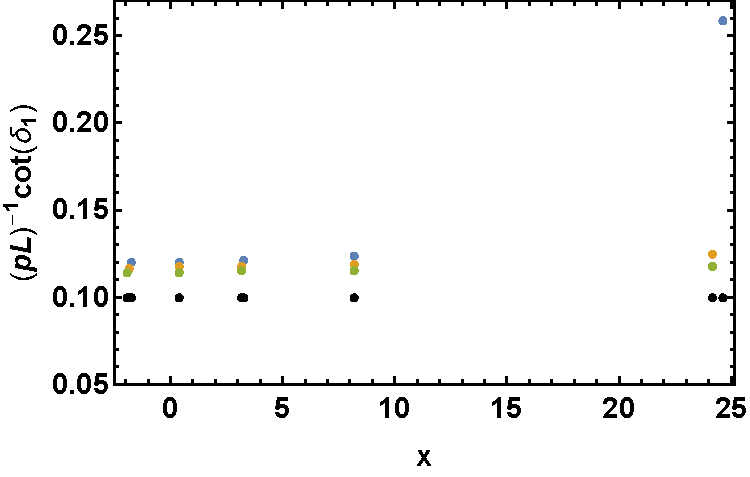
\includegraphics[width=.65\textwidth]{figure/luescher1d.pdf}
\caption{Results in 1-D using non-continuum eigenvalues $x=p^2L^2/4\pi^2$ of the Schr\"odinger equation with $N=10$, 12, and 14.  The interaction was tuned such that $a_{10}/L=.1$.  The non-black points are obtained using $S^\bigcirc_1(x)$ with $N=10$ being furthest from a flat line and $N=14$ being closest.  The black points are obtained using $S^{\dispersion}_1(x)$  and exhibit the correct flat-line behavior.  In addition to momentum-dependent terms, there is a constant offset, as is apparent when comparing the colored points with the black points.  The colored dashed lines are the derived induced momentum-dependent terms (see text).\todo{Need better figure.-T.L.}\label{fig:luescher1d}}
\end{figure}

We can derive the functional form of these induced momentum-dependent terms by extracting the contribution to the dispersion L\"uscher from the continuum L\"uscher.
\begin{align*}
 \frac{1}{2 \pi^{2}} S^\bigcirc_{1}\left(x\right)=\frac{1}{2 \pi^{2}} \sum_{n=-\infty}^{\infty} \frac{1}{n^{2}-x} &=\frac{1}{2 \pi^{2}} \sum_{n\in \operatorname{B.Z.}} \frac{1}{n^{2}-x} +\frac{1}{2 \pi^{2}} \sum_{n\notin \operatorname{B.Z.}} \frac{1}{n^{2}-x} \\
 &= \frac{1}{2 \pi^{2}} S^{\dispersion}_{1}\left(x\right)+\frac{1}{2 \pi^{2}} \sum_{n\notin \operatorname{B.Z.}} \frac{1}{n^{2}-x}\\
&=\frac{a_{10}}{L}+\frac{1}{2 \pi^{2}} \sum_{n\notin \operatorname{B.Z.}} \frac{1}{n^{2}-x} \ .
\end{align*}
where the energy in $x$ is a finite-spacing finite-volume $\nstep=\infty$ energy.
In the second term the sum is restricted to values of $n$ outside the Brillouin zone.
Assuming $n^2\gg x$, we can expand in powers or $x$,
\begin{equation}
    \frac{1}{2 \pi^{2}} \sum_{n=-\infty}^{\infty} \frac{1}{n^{2}-x}
        =
    \frac{a_{10}}{L}+\frac{1}{2 \pi^{2}} \sum_{n\notin \operatorname{B.Z.}} \frac{1}{n^{2}-x}
        =
    \frac{a_{10}}{L}+\frac{1}{2 \pi^{2}} \sum_{n\notin \operatorname{B.Z.}} \left(\frac{1}{n^2}+\frac{x}{n^4}+\frac{x^2}{n^6}+\mathcal{O}(x^3)\right)
\end{equation}
We make the replacement $\sum_{n\notin\operatorname{B.Z.}}\mapsto\left(\sum_{n=-\infty}^\infty-\sum_{n\in\operatorname{B.Z.}}\right)$, which allows each summation in the expansion to be determined term by term to arbitrary precision.

\begin{table}
    \caption{
    The induced momentum-dependent terms to order $x^2$ due to a contact interaction using $S^\bigcirc_1(x)$ as a function of discretization $N$.
    Here $x$ is determined by a finite-spacing finite-volume $\nstep=\infty$ eigenenergy.}
    \label{tab:induced terms in 1 d}
    \begin{tabular}{c|c}
    $N$
        &
            $\frac{1}{2 \pi^{2}} \sum_{n\notin \operatorname{B.Z.}} \left(\frac{1}{n^2}+\frac{x}{n^4}+\frac{x^2}{n^6}\right)$       \\
        \hline
    10  &   $0.020398280 + 0.00028079187 x + 7.1106444\times10^{-6} x^2$    \\
    12  &   $0.016964618 + 0.00016064496 x + 2.7825342\times10^{-6} x^2$    \\
    14  &   $0.014523490 + 0.00010045521 x + 1.2660940\times10^{-6} x^2$    \\
    \end{tabular}
\end{table}

\Tabref{induced terms in 1 d} shows these terms for $N=10$, 12, and 14.
The colored dashed lines in \Figref{luescher1d} correspond to the functions given in this table.  In the limit $N\mapsto\infty$ all terms vanish and one recovers the flat, momentum-independent behavior.
Of course, analyzing the finite-spacing dispersion zeta function $S^{\dispersion}_1$ with $\nstep=\infty$ produces the flat behavior all the way through.
This demonstrates that it was not the contact operator that caused the momentum dependence, but that the dependence was induced by leveraging the continuum finite-volume formalism itself.
